Let us investigate the number of prime factors of integers.

Figure~\ref{fig:scatter_plot_of_prime_factors} shows the number of prime
factors for each integer less than 100.

\begin{center}
    \begin{figure}[!hbtp]
        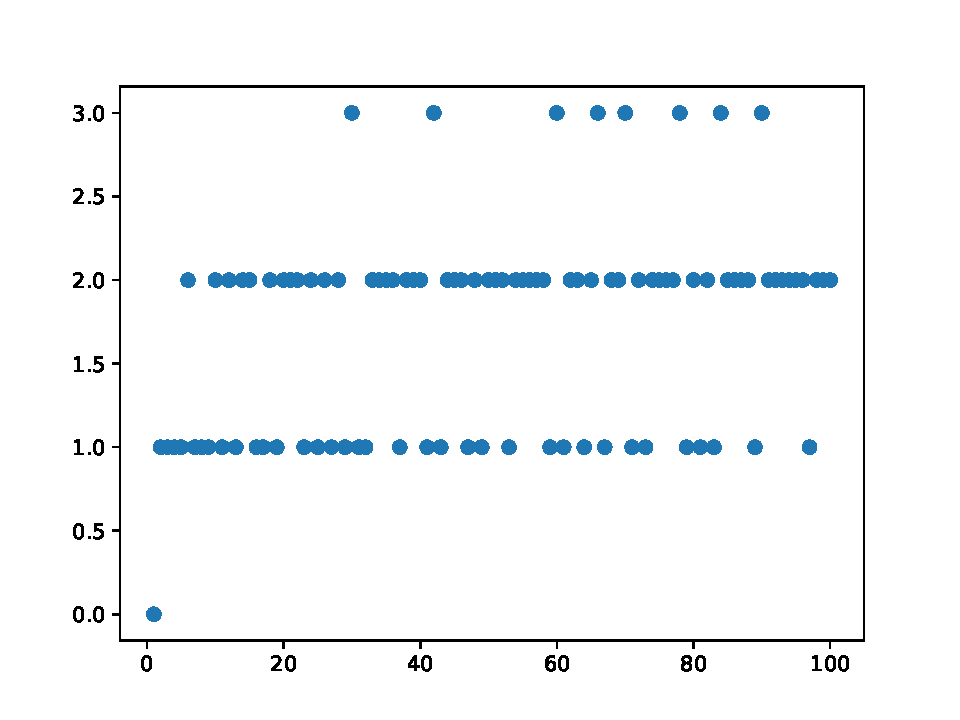
\includegraphics[width=5cm]{src/scatter_plot_of_prime_factors.pdf}
        \caption{The number of prime factors of each integer}
        \label{scatter_plot_of_prime_factors}
    \end{figure}
\end{center}

Table~\ref{tab:number_of_factors_table} shows these counts for \(95\leq
n\leq 100\).

\begin{center}
    \begin{table}[!hbtp]
        \begin{tabular}{rr}
\toprule
   N &  Number of factors \\
\midrule
  95 &                  2 \\
  96 &                  2 \\
  97 &                  1 \\
  98 &                  2 \\
  99 &                  2 \\
 100 &                  2 \\
\bottomrule
\end{tabular}

    \end{table}
\end{center}

The number with the most prime factors
has3 prime factors.

The number of factors is probably related to the number of primes which has
a lower bound given by:

\small
\[
\pi(n)=\frac{n}{\log{n}}=\frac{1}{n - 1} + \frac{13}{12} - \frac{1}{24} \left(n - 1\right)^{2} + \frac{11}{720} \left(n - 1\right)^{3} - \frac{11}{1440} \left(n - 1\right)^{4} + \frac{271}{60480} \left(n - 1\right)^{5} + \frac{5 n}{12} + \mathcal{O}\left(\left(n - 1\right)^{6}; n\rightarrow 1\right)
\]
